% Tento soubor nahraďte vlastním souborem s přílohami (nadpisy níže jsou pouze pro příklad)

% Pro kompilaci po částech (viz projekt.tex), nutno odkomentovat a upravit
%\documentclass[../projekt.tex]{subfiles}
%\begin{document}

% Umístění obsahu paměťového média do příloh je vhodné konzultovat s vedoucím
%\chapter{Obsah přiloženého paměťového média}

\chapter{Příklady zdrojových kódů v~jazyce Koubp a~jejich AST reprezentace}

\section{Příkaz if-elseif}
\begin{lstlisting}[language=Koubp]
    if (vyraz)
        prikaz();
    elseif(vyraz)
        prikaz();
\end{lstlisting}
\begin{figure}[ht]
    \centering
    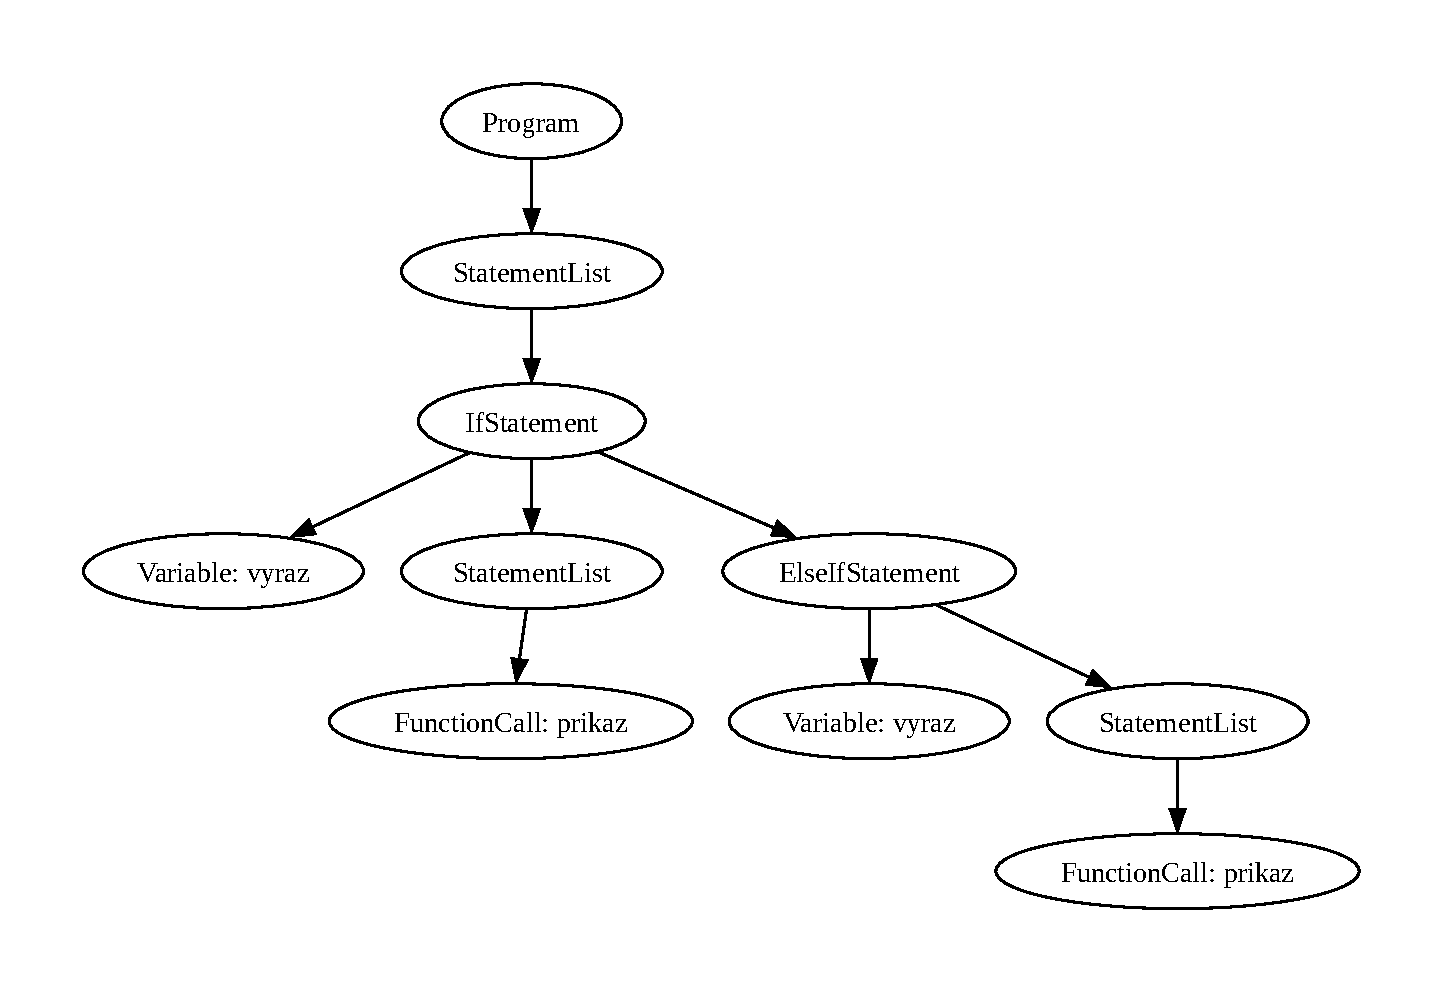
\includegraphics[width=\textwidth]{obrazky-figures/ast_if_elseif.pdf}
    \caption{Programem vygenerovaný AST pro konstrukci \texttt{if-elseif}}
    \label{fig_ast_elseif}
\end{figure}

\section{Příkaz if-else if}
\begin{lstlisting}[language=Koubp]
    if (vyraz)
        prikaz();
    else if(vyraz)
        prikaz();
\end{lstlisting}
\begin{figure}[ht]
    \centering
    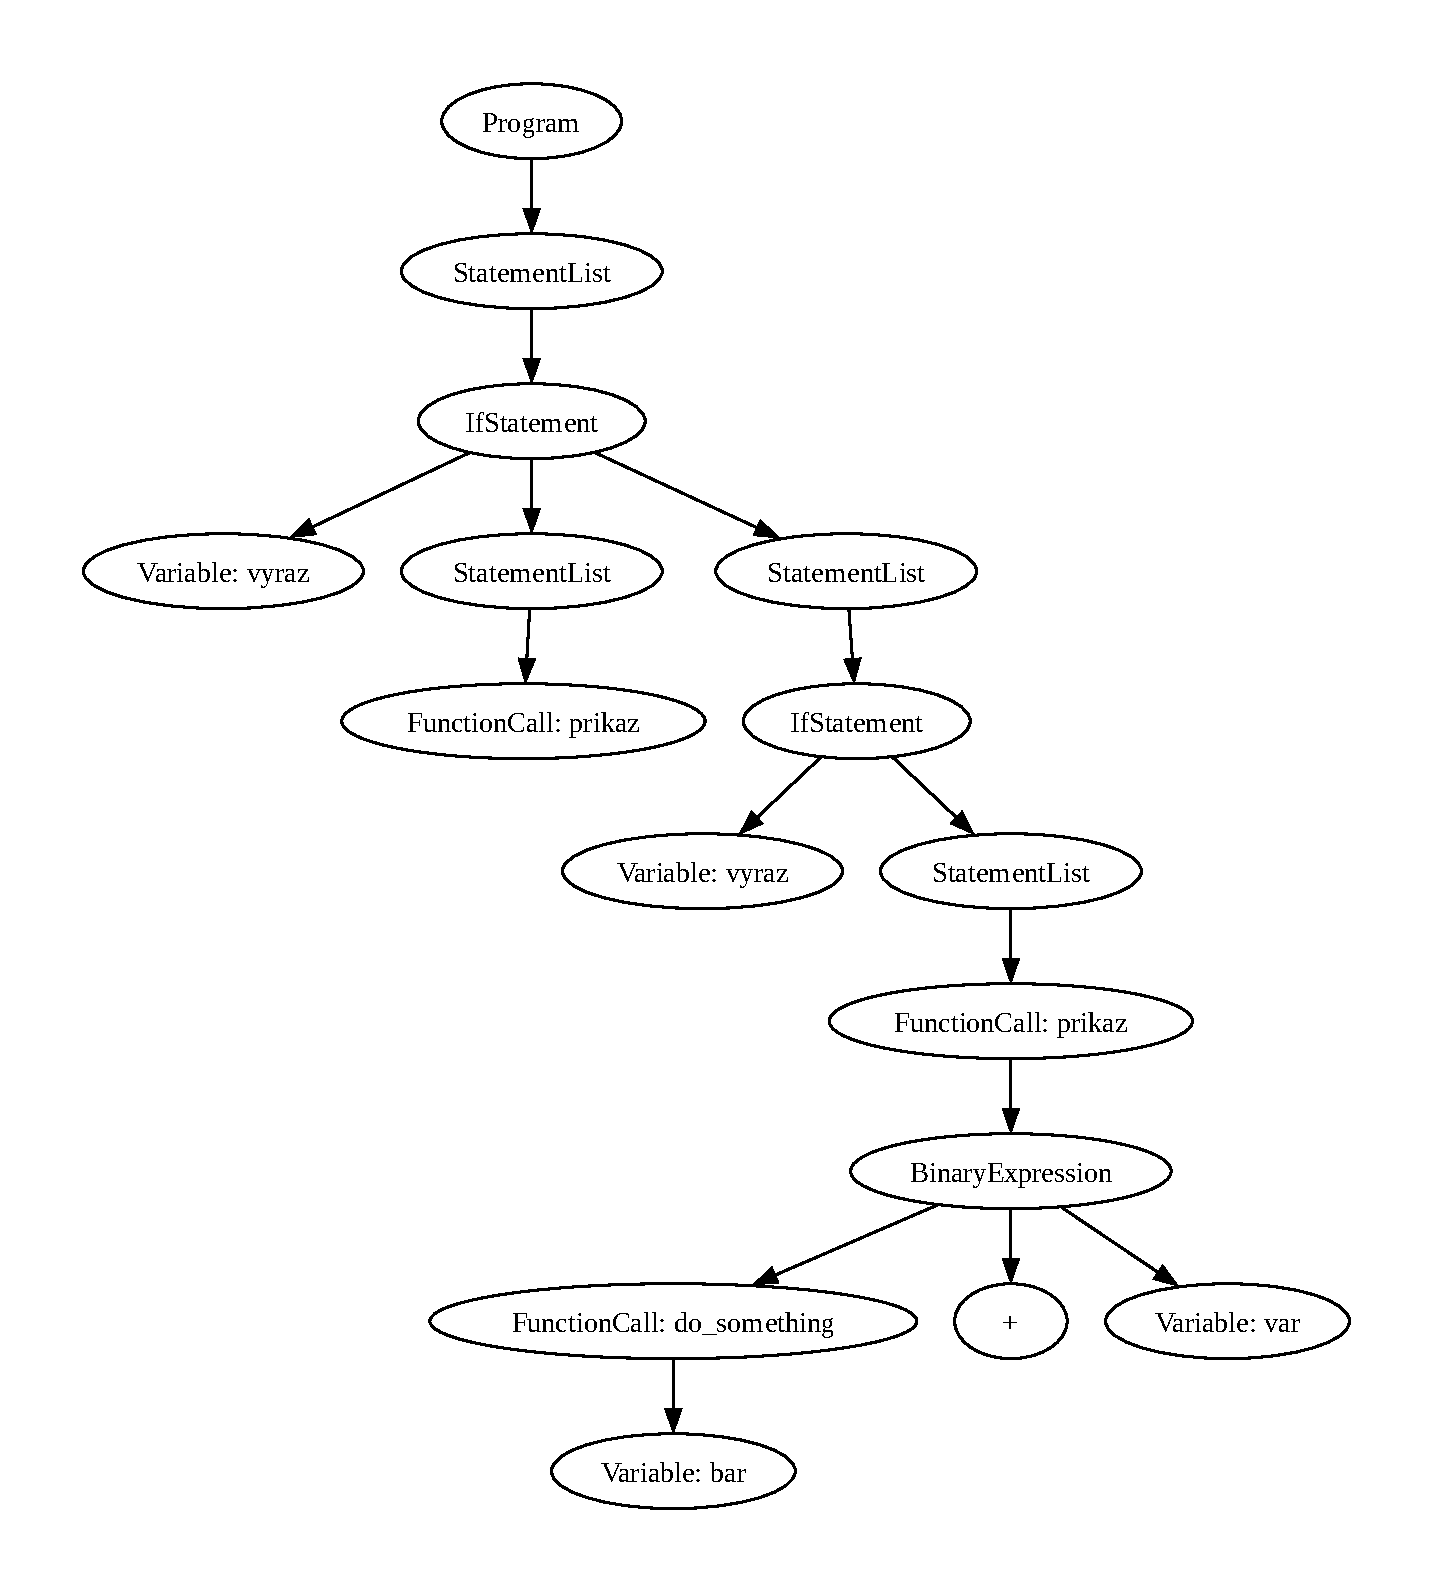
\includegraphics[width=\textwidth]{obrazky-figures/ast_if_else_if.pdf}
    \caption{Programem vygenerovaný AST pro konstrukci \texttt{if-else if}}
    \label{fig_ast_else_if}
\end{figure}

\newpage
\section{For cyklus}

\begin{lstlisting}[language=Koubp]
    for (int i = 0; i < 2; i = i + 1) {}
\end{lstlisting}
\begin{figure}[h]
    \centering
    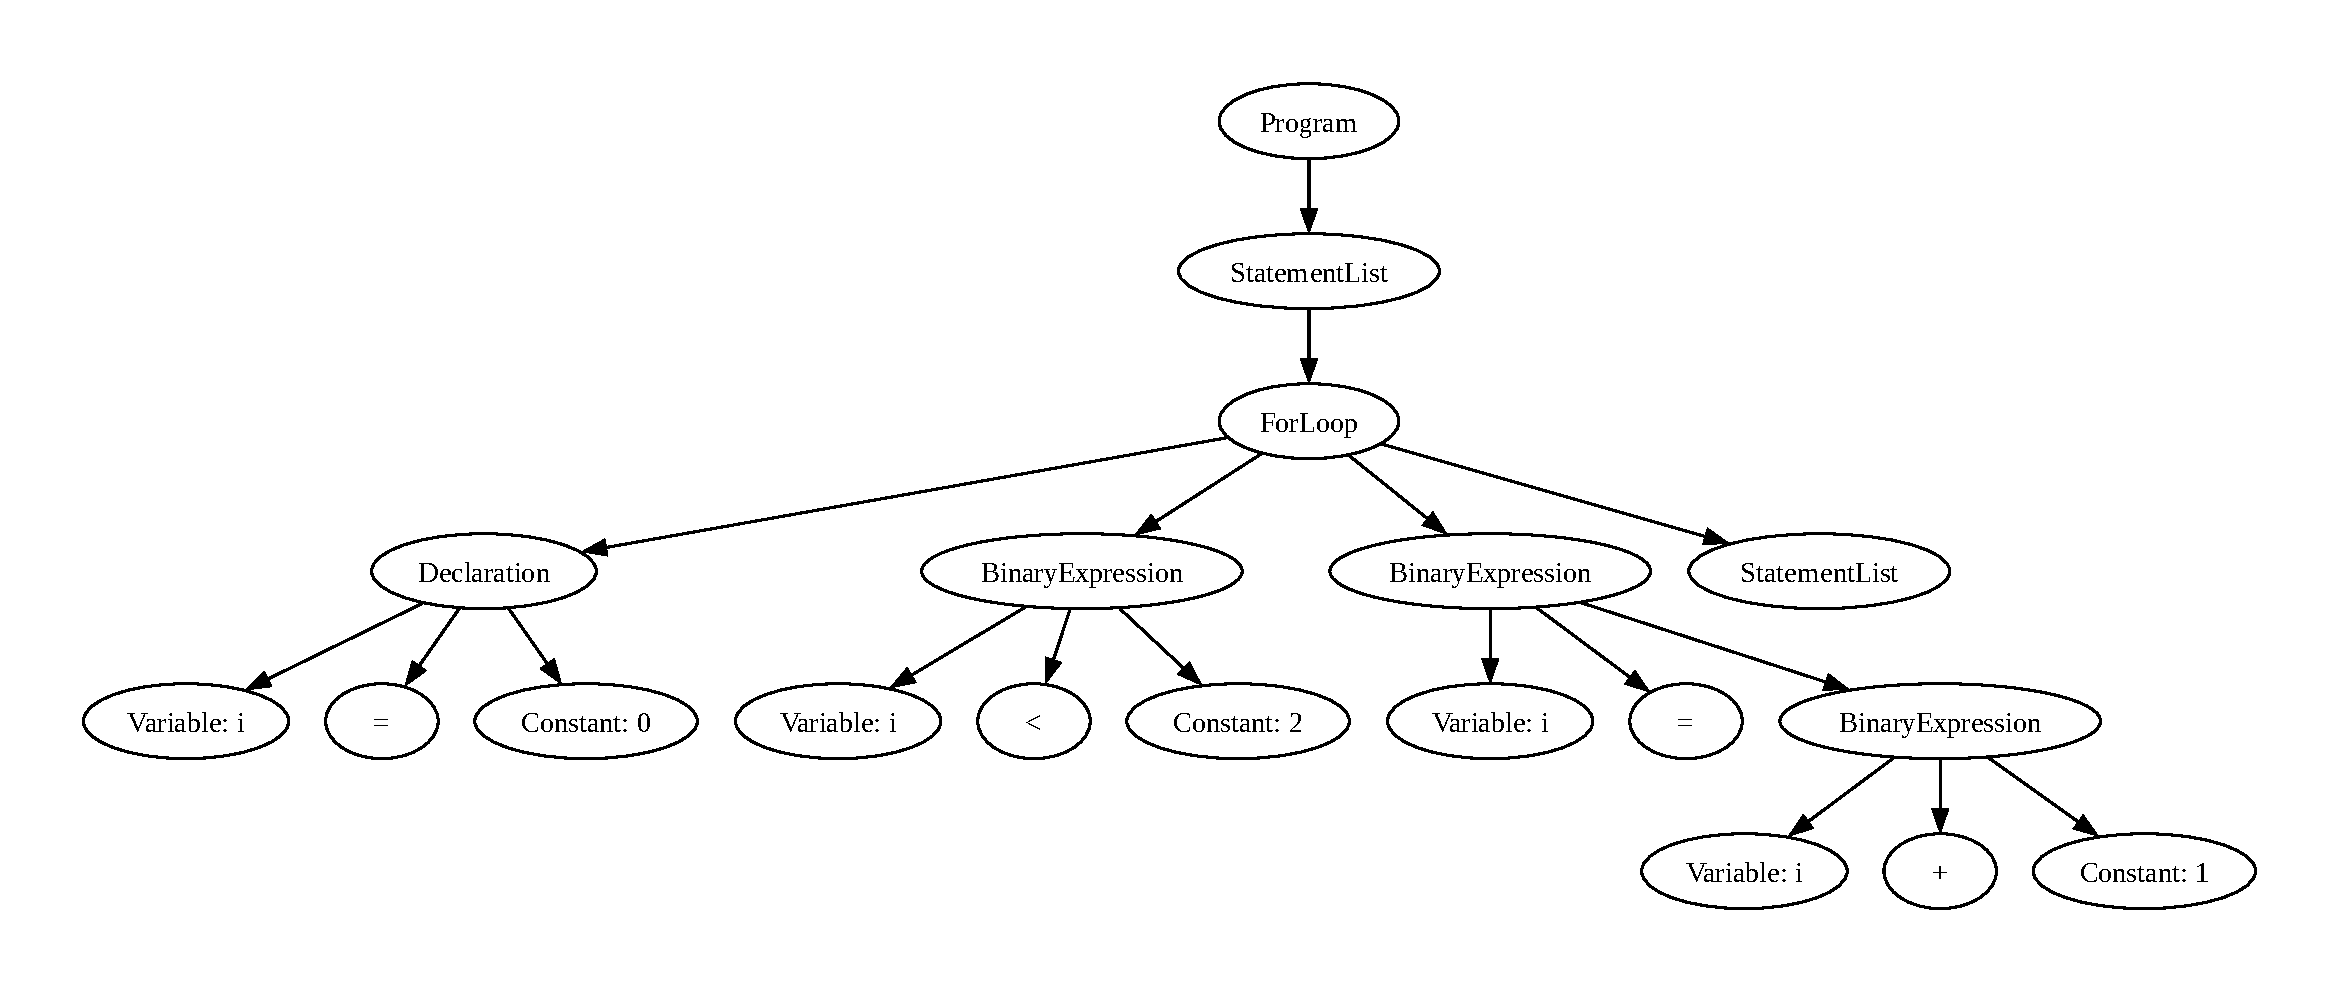
\includegraphics[width=\textwidth]{obrazky-figures/tree_for.pdf}
    \caption{Programem vygenerovaný AST pro cyklus \texttt{for}.}
    \label{fig_ast_for}
\end{figure}
\newpage
\section{Deklarace a přiřazení}

\begin{lstlisting}[language=Koubp]
    float input = do_something(var, f(1) + 2) + 20.0*d;
\end{lstlisting}
\begin{figure}[h]
    \centering
    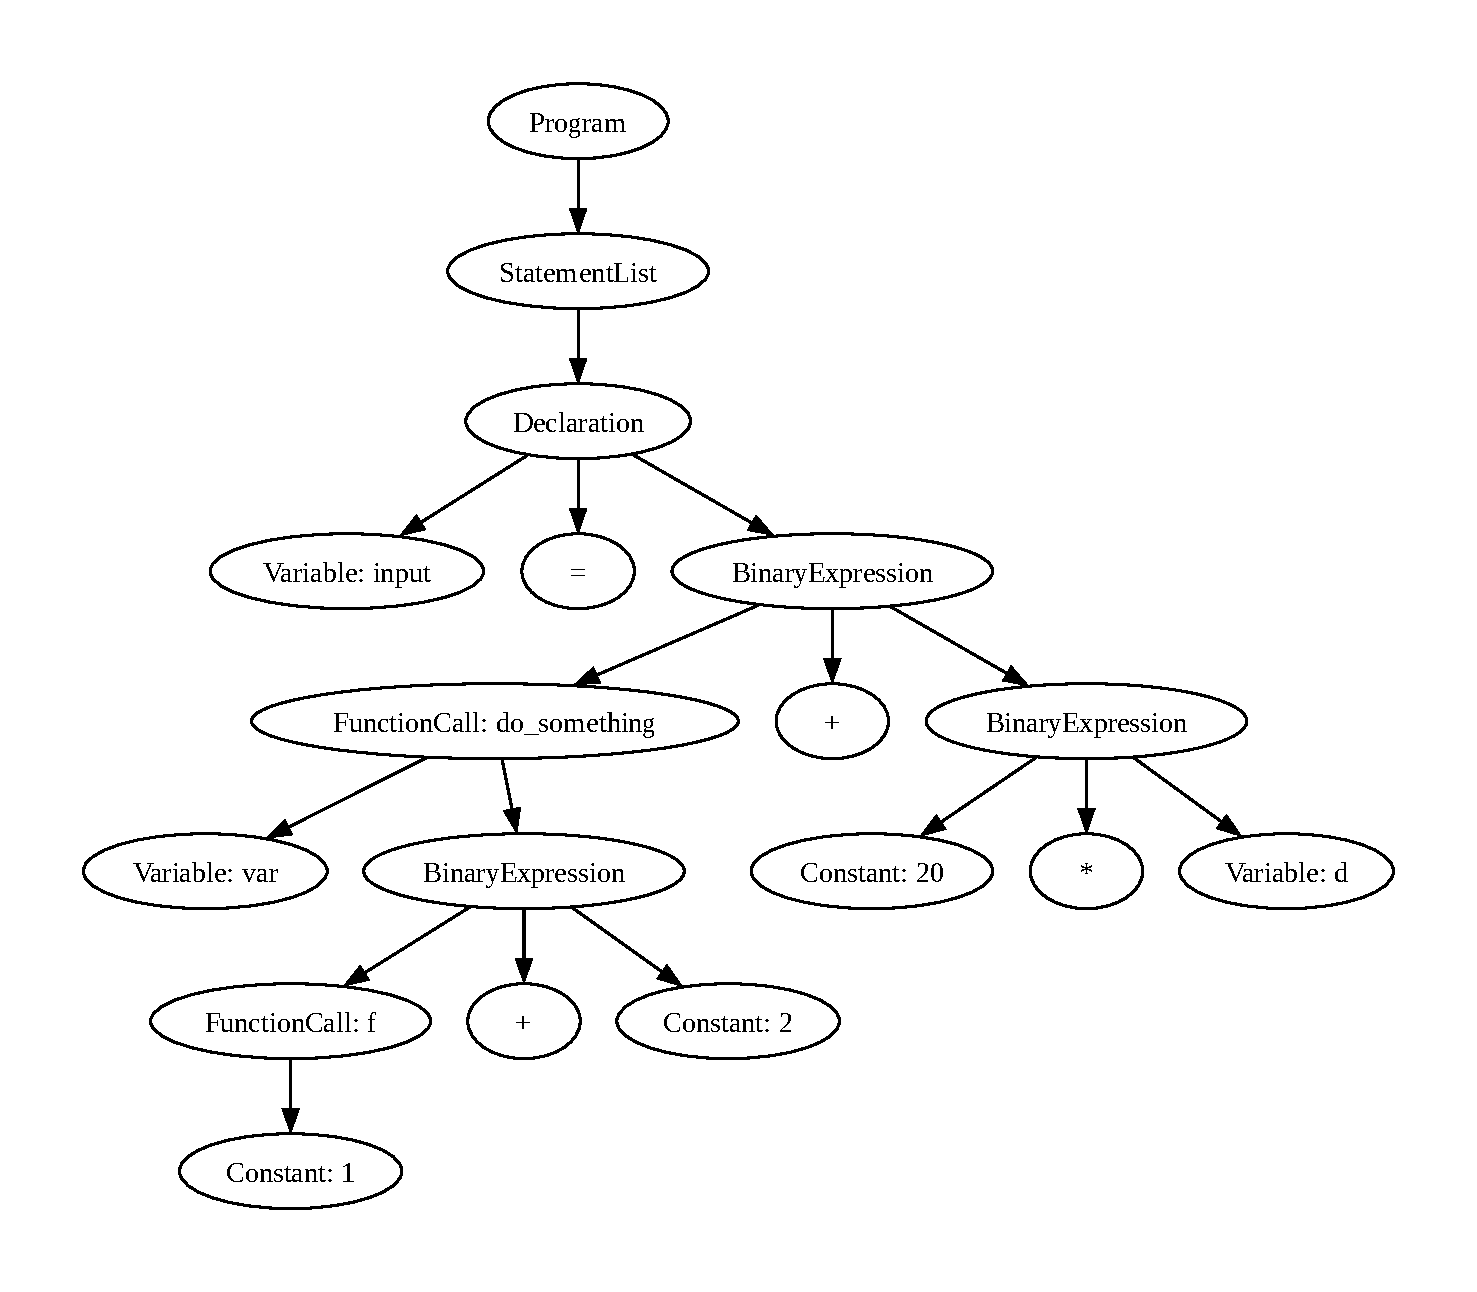
\includegraphics[width=\textwidth]{obrazky-figures/tree_deklarace.pdf}
    \caption{Programem vygenerovaný AST pro deklaraci s~přiřazením.}
    \label{fig_ast_declaration}
\end{figure}


\chapter{Třídní diagram popisující vztahy tříd provádějící syntaktickou analýzu}\label{kap_priloha_b}

Diagram obsahuje pouze třídy, které se starají o~algoritmus syntaktické analýzy, respektive simulaci zásobníkového automatu.
Další pomocné třídy, jako například LL tabulka nebo precedenční tabulka, nejsou do grafu přidány kvůli přehlednosti  vzhledem k~velikosti diagramu.
\begin{figure}[ht]
    \centering
    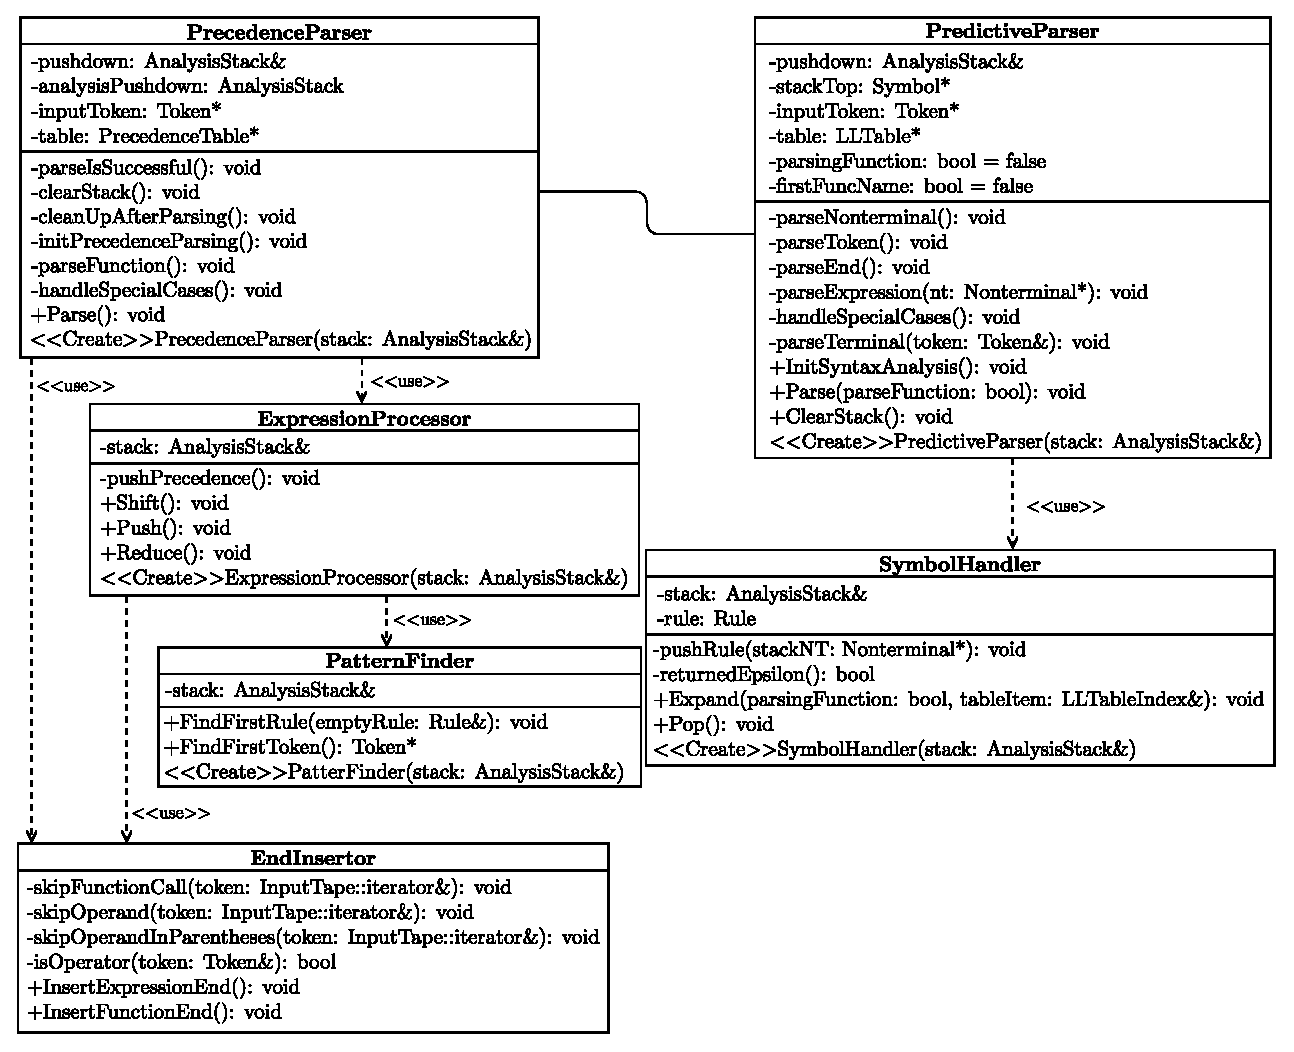
\includegraphics[width=0.92\textwidth]{obrazky-figures/class_diagram.eps}
    \caption{Vztahy mezi třídami, které spolupracují na syntaktické analýze.}
\end{figure}

\chapter{Třídní hierarchie uzlů AST} \label{kap_priloha_c}
Pro větší přehlednost je hierarchie rozdělena do dvou obrázků.
\begin{figure}[h]
    \centering
    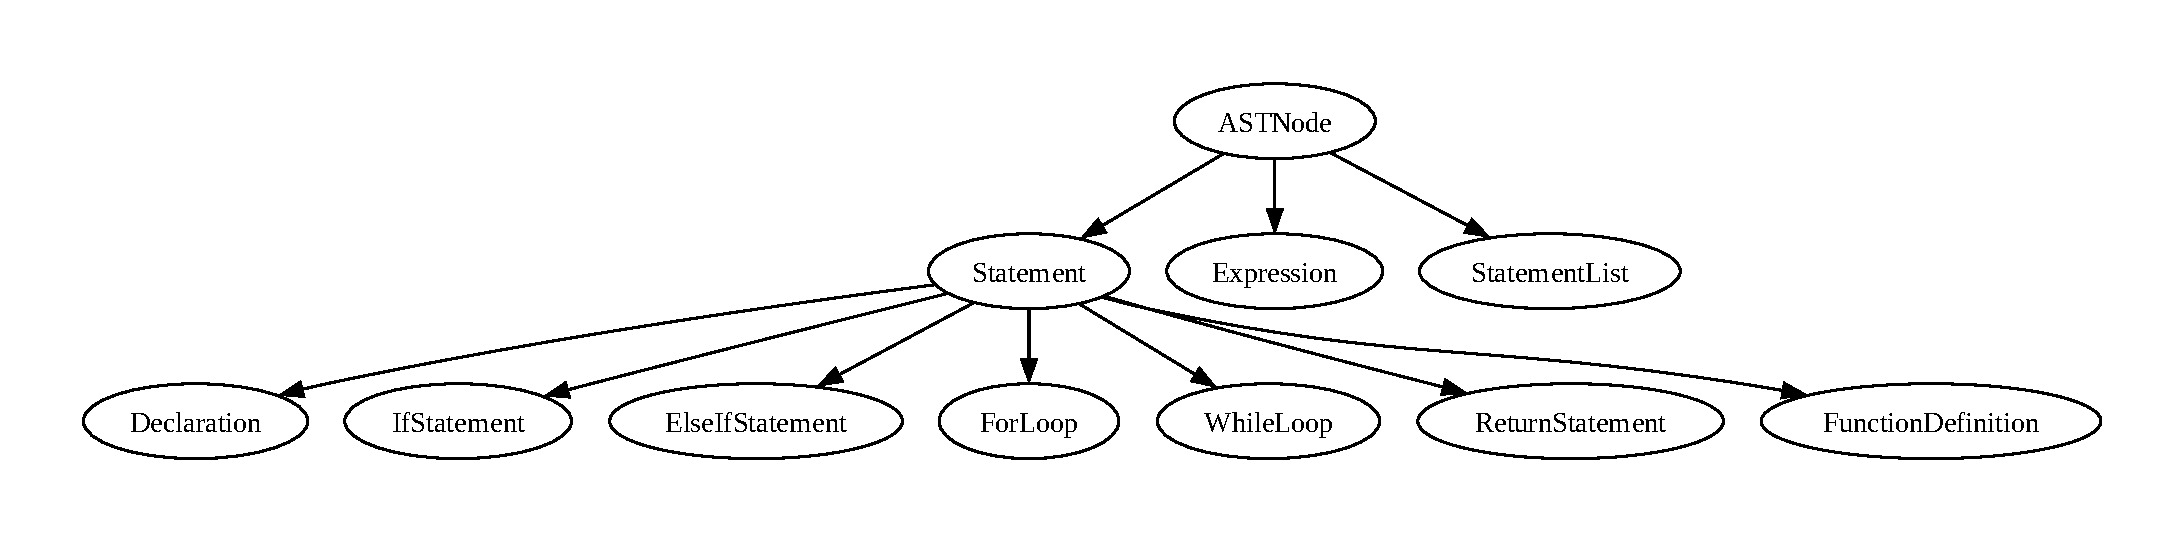
\includegraphics[width=\textwidth]{obrazky-figures/hierarchy_statement.pdf}
    \caption{Třídní hierarchie s~třídami reprezentujícími jednotlivé příkazy v~AST.}
    \label{fig_hierarchie_statement}
\end{figure}

\begin{figure}[h]
    \centering
    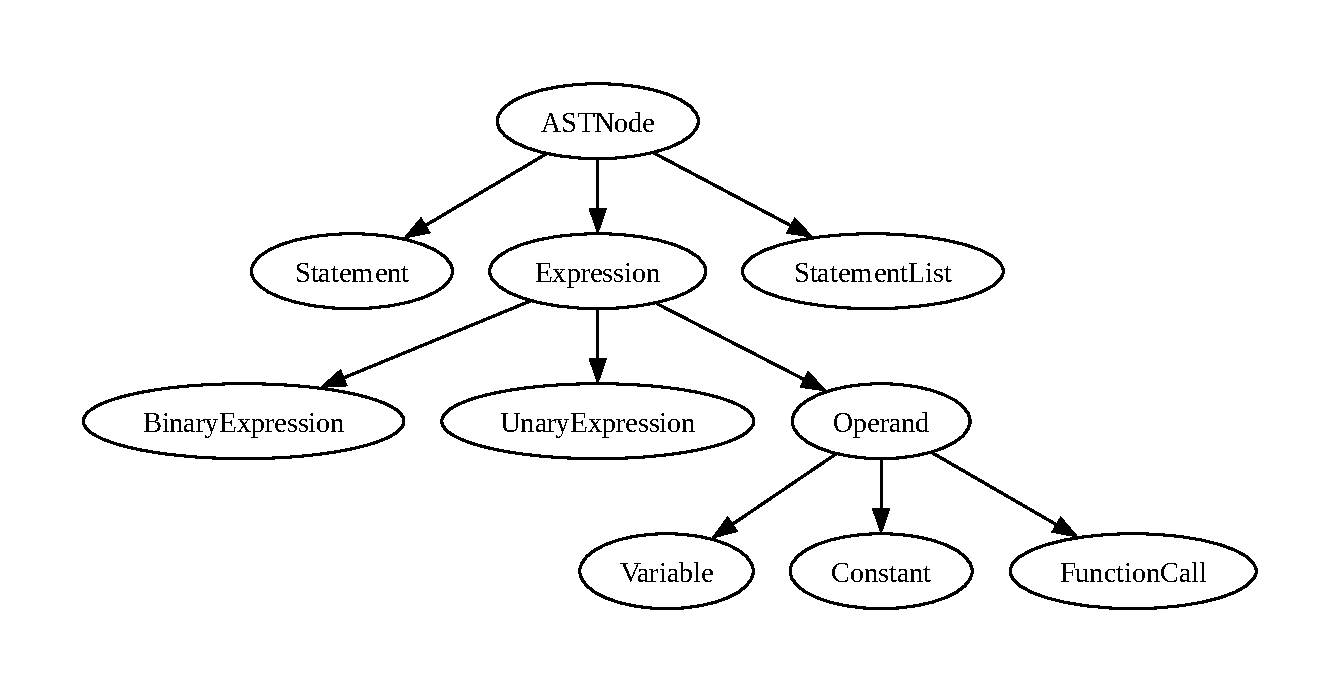
\includegraphics[width=\textwidth]{obrazky-figures/hierarchy_expression.pdf}
    \caption{Třídní hierarchie s~třídami reprezentujícími jednotlivé typy výrazů v~AST.}
    \label{fig_hierarchie_expression}
\end{figure}


%\chapter{Plakát}



% Pro kompilaci po částech (viz projekt.tex) nutno odkomentovat
%\end{document}
